\begin{figure*}
\inclGrid{spl-input}
\caption{Nine of the lens candidates marked up with spaghetti
  diagrams.  Red, blue and green dots are proposed locations for
  maxima, minima and saddle points of the arrival time respectively.
  The curves help guide the placement of the dots, but their precise
  appearance has no significance.  This selection includes the
  best-modelled systems, but also one case (SW57 at upper right) of
  unsuccessful modelling.  Since the modelling process is
  collaborative among the volunteers, with anyone welcome to
  contribute new models or modify existing ones, there are variant
  spaghetti diagrams for all the modelled systems.  The online
  supplement displays all the models presented for discussion during
  this work.
\label{fig:splinput}}
\end{figure*}

\begin{figure*}
\inclGrid{arrival_spaghetti}
\caption{Arrival-time surfaces for models of the systems from
  Figure~\ref{fig:splinput}.  The registration differs slightly from
  Figure~\ref{fig:splinput}, but the coloured dots represent exactly
  the sky positions specified in the earlier figure.  The orange
  contours only qualitatively resemble the earlier pink curves, as
  they are now precise saddle-point contours from lens models.
  \label{fig:arriv}}
\end{figure*}

\begin{figure*}
\inclGrid{nsynth}
\caption{Synthetic images of the systems from
  Figure~\ref{fig:splinput}, derived from the lens models.  The
  reconstructed lensed features are keep the Space~Warps false-colour
  scheme from Figures~\ref{fig:splinput}.  The rest has been changed
  to black-and-white.
  \label{fig:synth}}
\end{figure*}


\begin{figure*}
\inclGrid{kappa_map_interpol}
\caption{Ensemble-average mass distribution $\kappa$ for which the
  results Figures~\ref{fig:arriv}--\ref{fig:synth} were derived.  The
  dashed curves denote $\kappa=1$.  Most of the mass maps have a
  $180^\circ$-rotation symmetry, which is imposed by default.  For
  SW02 and SW57, where the lensing mass is clearly asymmetric, the
  modeller chose to turn off the symmetry.
\label{fig:kappa}}
\end{figure*}

\begin{figure*}
\inclGrid{kappa_encl}
\caption{Cumulative circular-averages of the mass maps from
  Figure~\ref{fig:kappa}, with uncertainties.  More precisely, we show
  the enclosed mass within a given projected radius, expressed as the
  mean $\kappa$ with a given number of arcsec from the centre of the
  lensing galaxy.  The orange bands refer to the full ensemble of mass
  maps for the models, while the red curves show the ensemble
  averages.  The dashed vertical line indicates the notional Einstein
  radius, or where the mean enclosed $\kappa$ is unity.  The short
  vertical arrows marks the positions of the images (maxima, saddle
  points and minima).
  \label{fig:encl}}
\end{figure*}


\begin{figure*}
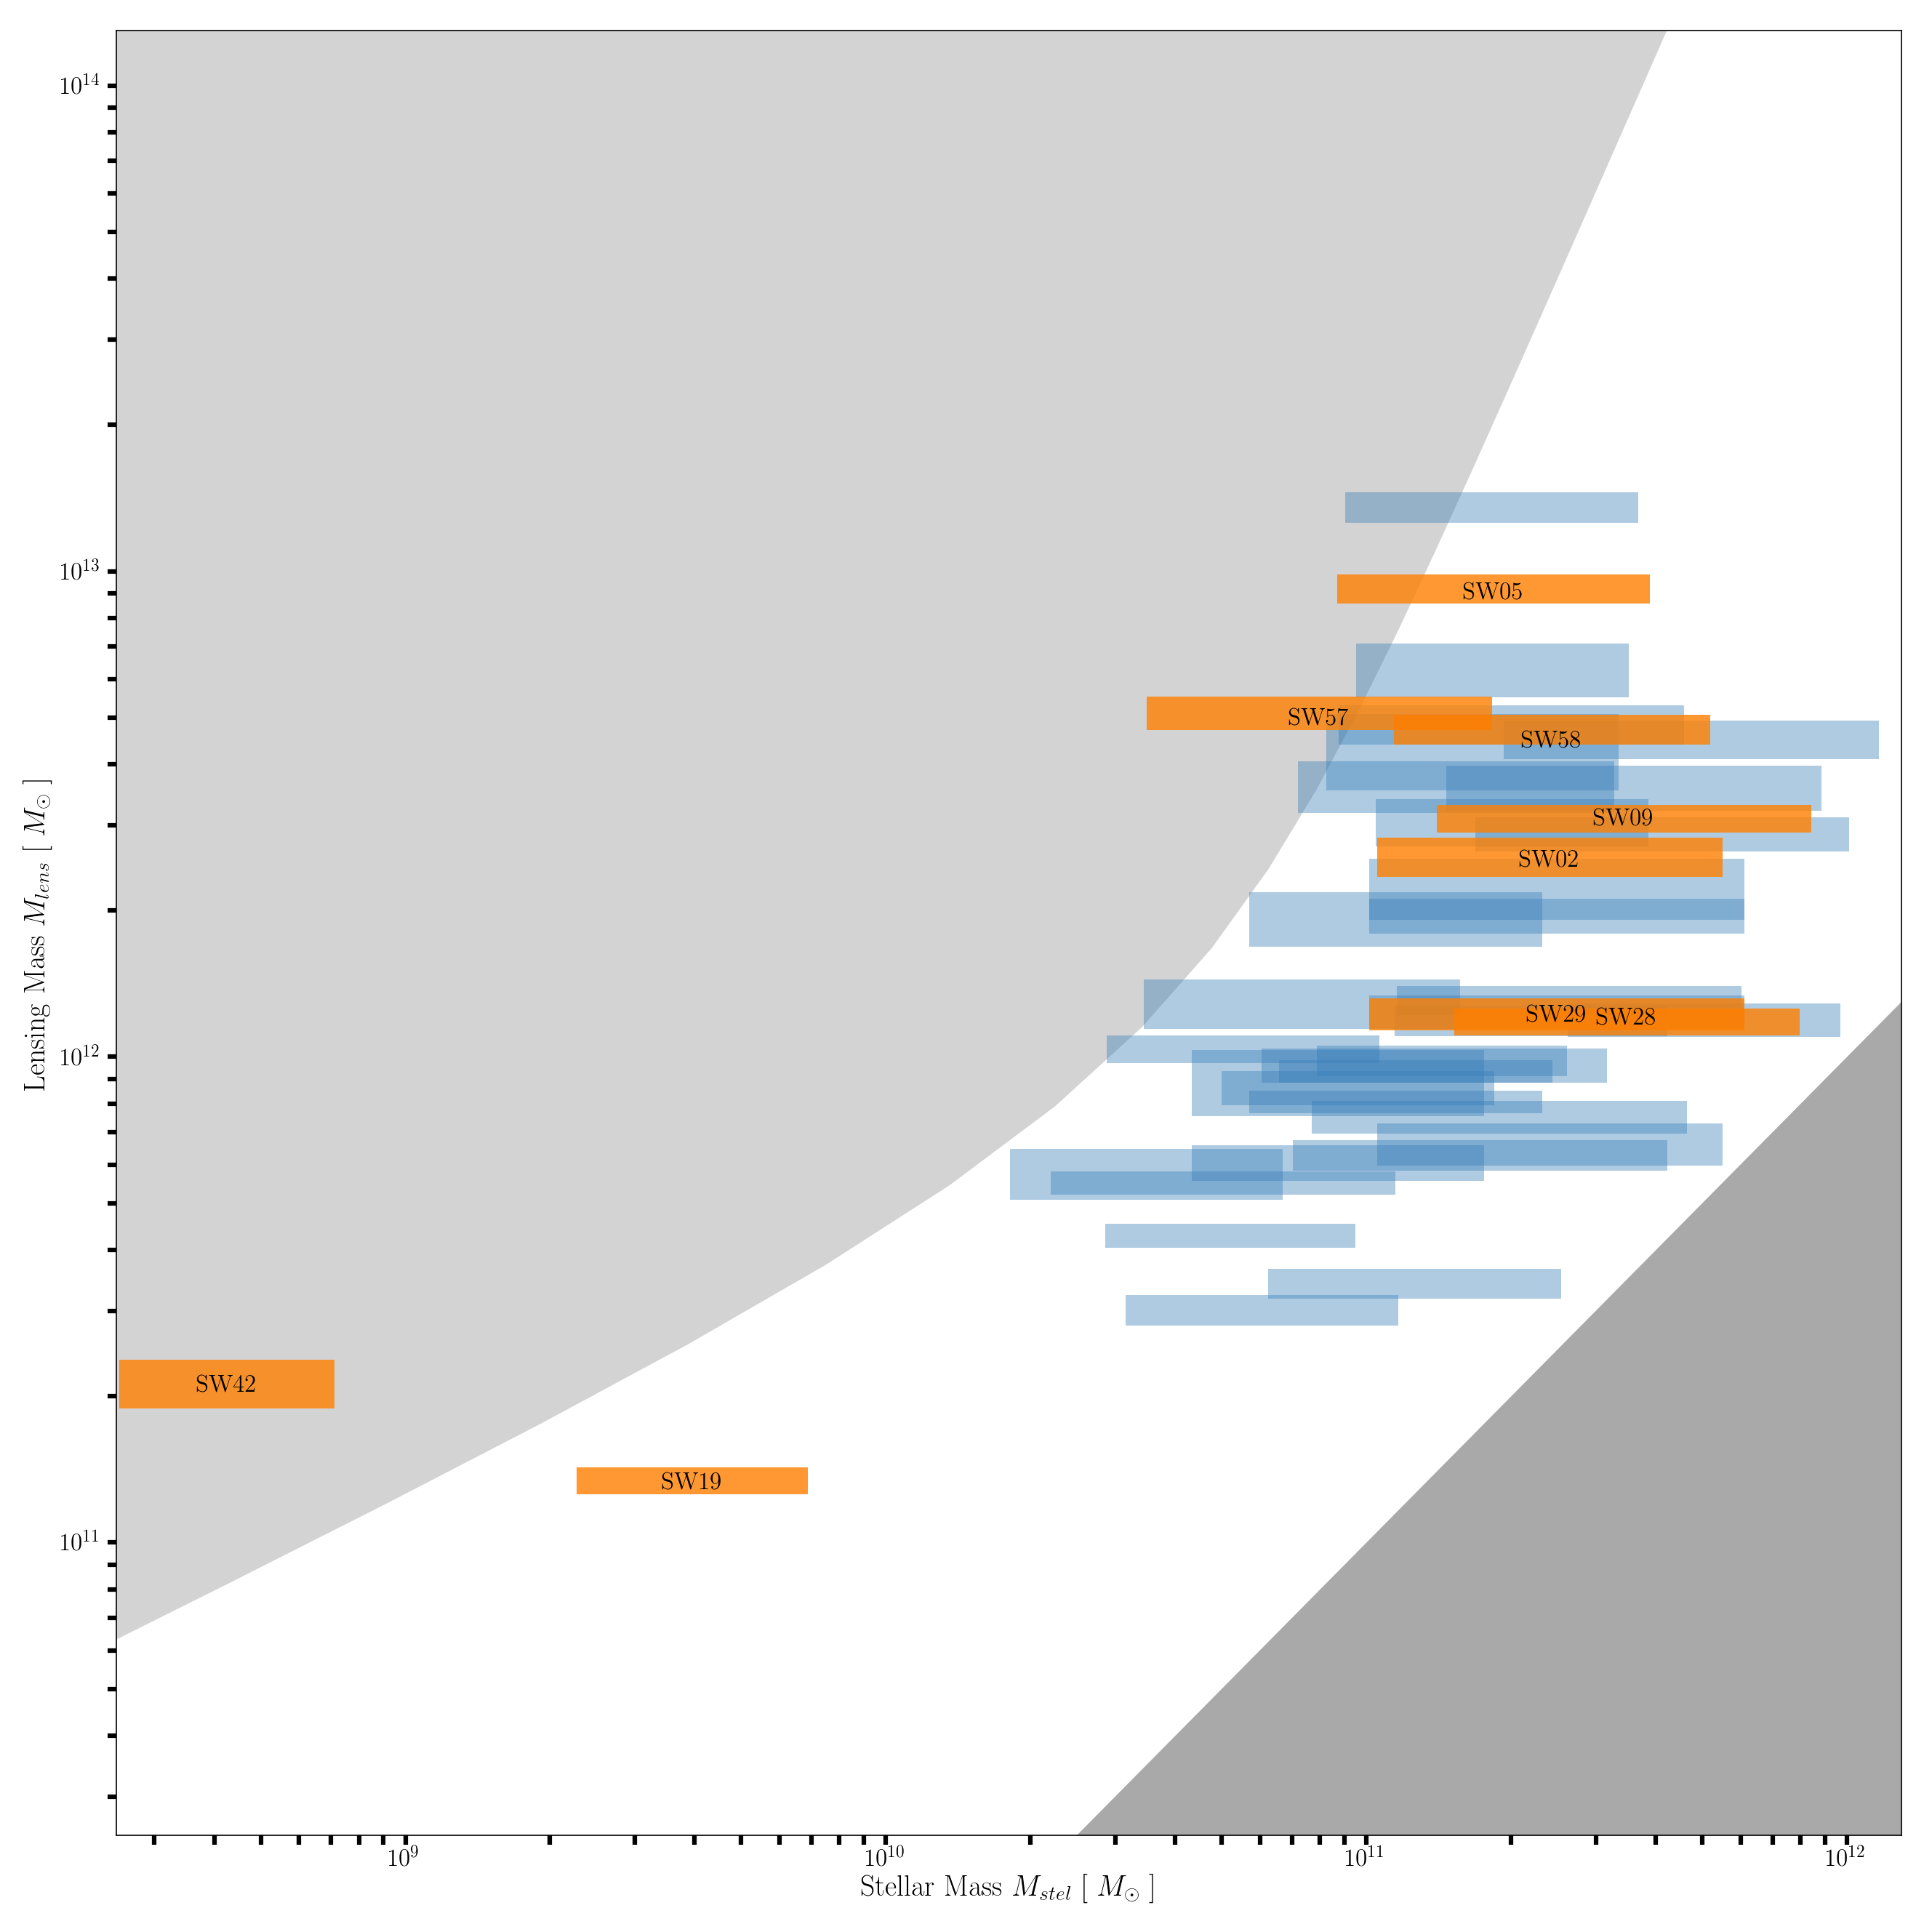
\includegraphics[width=\linewidth]{img/mlens_vs_mstel_one/mstel_vs_mtot_one}
\caption{Total mass in the model against the estimated stellar mass,
  alongside the values for the whole sample.  (The labelled orange
  bars are the systems shown in detail in
  Figures~\ref{fig:splinput}--\ref{fig:encl}.)  The lower-right shaded
  region is unphysical according to the stellar-population models,
  because it gives $M<\Mstel$. The upper-left shaded region is
  unphysical according to abundance matching (see
  Section~\ref{sec:stellar-mass}) because it gives $M>\Mhalo$.  That
  is to say, the unshaded region is
  $0<\haloindex<1$. \label{fig:stelmass}}
\end{figure*}


\begin{table*}
  \caption{Diagnostics of a selected model for each Space Warps candidate
    (see Section~\ref{sec:summary}).}
  \label{tab:models}
  
\begin{tabular}{c c c | c | c c c | c | c c | c c c}
  \hline
  SWID & ZooID & CFHTLS Name
  
    & \rot{$z_\text{lens}$}

    & \multicolumn{1}{l}{\rot{\shortstack[l]{unblended\\images}}}
    & \rot{\shortstack[l]{all images\\discernible\,}}
    & \rot{\shortstack[l]{isolated\\lens}}

    & \rot{\shortstack[l]{image\\morpho-\\logy}}
    
    & \rot{\shortstack[l]{synthetic\\image\\reasonable}}
    & \rot{\shortstack[l]{mass map\\reasonable}}

    & \rot{\shortstack[l]{$\log_{10}\frac{\Mstel}{\Msun}$}\hskip-1.5pt}
    & \rot{\shortstack[l]{$\log_{10}\frac{M_\text{lens}}{\Msun}$}\hskip-2.2pt}
    & \rot{\shortstack[l]{halo-\\matching\\index $\haloindex$}}
  \\ \hline
 \sw{01} & \asw{4dv8} & J022409.5$-$105807 & \UK
    & \NO & \NO & \NO & LQ & \OK & \OK
    & \UK & \UK & \UK   \\
    
 \sw{02} & \asw{619d} & J140522.2$+$574333 & 0.7
    & \NO & \OK & \NO & SQ & \OK & \OK
    & 11.4 & 12.4 & 0.47   \\
    
 \sw{03} & \asw{6mea} & J142603.2$+$511421 & \UK
    & \OK & \NO & \NO & D & \OK & \OK
    & \UK & \UK & \UK   \\
    
 \sw{04} & \asw{9cjs} & J142934.2$+$562541 & 0.5
    & \OK & \NO & \NO & D & \NO & \OK
    & 11.3 & 13.1 & 0.93   \\
    
 \sw{05} & \asw{7k4r} & J143454.4$+$522850 & 0.58
    & \OK & \OK & \OK & IQ & \OK & \OK
    & 11.3 & 13.0 & 0.83   \\
    
 \sw{06} & \asw{8swn} & J143627.9$+$563832 & 0.5
    & \NO & \OK & \OK & SQ & \OK & \NO
    & 11.1 & 11.9 & 0.46   \\
    
 \sw{07} & \asw{7e08} & J220256.8$+$023432 & \UK
    & \OK & \OK & \NO & D & \OK & \OK
    & \UK & \UK & \UK   \\
    
 \sw{08} & \asw{99ed} & J020648.0$-$065639 & 0.8
    & \OK & \OK & \NO & D & \OK & \OK
    & 11.4 & 12.3 & 0.40   \\
    
 \sw{09} & \asw{2asp} & J020832.1$-$043315 & 1.0
    & \NO & \OK & \OK & SQ & \OK & \OK
    & 11.5 & 12.5 & 0.40   \\
    
 \sw{10} & \asw{2bmc} & J020848.2$-$042427 & 0.8
    & \OK & \NO & \OK & D & \NO & \NO
    & 11.3 & 11.9 & 0.29   \\
    
 \sw{11} & \asw{2qtn} & J020849.8$-$050429 & 0.8
    & \NO & \OK & \NO & LQ & \OK & \OK
    & 11.2 & 11.8 & 0.29   \\
    
 \sw{12} & \asw{3wsu} & J022406.1$-$062846 & 0.4
    & \OK & \OK & \NO & D & \OK & \OK
    & 10.8 & 11.5 & 0.44   \\
    
 \sw{13} & \asw{47ae} & J022805.6$-$051733 & 0.4
    & \NO & \NO & \NO & SQ & \NO & \NO
    & 11.1 & 11.9 & 0.46   \\
    
 \sw{14} & \asw{4xjk} & J023123.2$-$082535 & \UK
    & \NO & \NO & \NO & SQ & \NO & \OK
    & \UK & \UK & \UK   \\
    
 \sw{15} & \asw{4nan} & J084841.0$-$045237 & 0.3
    & \NO & \OK & \NO & CQ & \OK & \OK
    & 10.7 & 11.6 & 0.59   \\
    
 \sw{16} & \asw{9bp2} & J140030.2$+$574437 & 0.4
    & \NO & \NO & \OK & D & \NO & \OK
    & 11.3 & 12.1 & 0.34   \\
    
 \sw{17} & \asw{5rnb} & J140622.9$+$520942 & 0.7
    & \OK & \NO & \NO & D & \NO & \OK
    & 11.1 & 12.0 & 0.44   \\
    
 \sw{18} & \asw{7hu2} & J143658.1$+$533807 & 0.7
    & \OK & \NO & \OK & D & \NO & \NO
    & 11.4 & 12.1 & 0.31   \\
    
 \sw{19} & \asw{1ld7} & J020642.0$-$095157 & 0.2
    & \NO & \OK & \NO & IQ & \NO & \OK
    &  9.6 & 11.1 & 0.84   \\
    
 \sw{20} & \asw{2dx7} & J021221.1$-$105251 & 0.3
    & \OK & \OK & \OK & D & \NO & \OK
    & 11.2 & 12.0 & 0.44   \\
    
 \sw{21} & \asw{4m3x} & J022533.3$-$053204 & 0.5
    & \OK & \NO & \NO & D & \NO & \OK
    & 11.1 & 11.5 & 0.24   \\
    
 \sw{22} & \asw{9ab8} & J022716.4$-$105602 & 0.4
    & \NO & \NO & \NO & D & \NO & \OK
    & 11.7 & 12.1 & 0.15   \\
    
 \sw{23} & \asw{3r61} & J023008.6$-$054038 & 0.6
    & \NO & \OK & \NO & LQ & \NO & \OK
    & 11.2 & 12.6 & 0.71   \\
    
 \sw{24} & \asw{50sk} & J023315.2$-$042243 & 0.7
    & \NO & \OK & \NO & D & \OK & \OK
    & 11.4 & 11.8 & 0.19   \\
    
 \sw{25} & \asw{07mq} & J090308.2$-$043252 & \UK
    & \NO & \NO & \OK & D & \NO & \OK
    & \UK & \UK & \UK   \\
    
 \sw{26} & \asw{5ma2} & J135755.8$+$571722 & 0.8
    & \OK & \NO & \OK & D & \NO & \NO
    & 11.4 & 12.3 & 0.43   \\
    
 \sw{27} & \asw{6jh5} & J141432.9$+$534004 & 0.7
    & \NO & \NO & \NO & LQ & \NO & \OK
    & 10.7 & 11.7 & 0.67   \\
    
 \sw{28} & \asw{7xrs} & J143055.9$+$572431 & 0.7
    & \NO & \OK & \NO & LQ & \OK & \OK
    & 11.5 & 12.1 & 0.23   \\
    
 \sw{29} & \asw{8qsm} & J143838.1$+$572647 & 0.8
    & \NO & \OK & \OK & SQ & \OK & \OK
    & 11.4 & 12.1 & 0.31   \\
    
 \sw{30} & \asw{2p8y} & J021057.9$-$084450 & \UK
    & \OK & \NO & \NO & IQ & \NO & \NO
    & \UK & \UK & \UK   \\
    
 \sw{31} & \asw{21r0} & J021514.6$-$092440 & 0.7
    & \NO & \OK & \NO & LQ & \OK & \OK
    & 11.3 & 12.7 & 0.65   \\
    
 \sw{32} & \asw{4iye} & J022359.8$-$083651 & \UK
    & \NO & \OK & \NO & IQ & \OK & \OK
    & \UK & \UK & \UK   \\
    
 \sw{33} & \asw{3s0m} & J022745.2$-$062518 & 0.6
    & \OK & \OK & \NO & D & \NO & \OK
    & 10.9 & 12.1 & 0.77   \\
    
 \sw{34} & \asw{51ld} & J023453.5$-$093032 & 0.5
    & \NO & \NO & \OK & D & \NO & \OK
    & 10.9 & 11.9 & 0.59   \\
    
 \sw{35} & \asw{4wgd} & J084833.2$-$044051 & 0.8
    & \NO & \OK & \NO & LQ & \OK & \OK
    & 11.4 & 12.1 & 0.32   \\
    
 \sw{36} & \asw{096t} & J090248.4$-$010232 & 0.4
    & \OK & \OK & \NO & D & \NO & \OK
    & 11.0 & 12.0 & 0.56   \\
    
 \sw{37} & \asw{86xq} & J143100.2$+$564603 & \UK
    & \NO & \NO & \OK & SQ & \OK & \OK
    & \UK & \UK & \UK   \\
    
 \sw{38} & \asw{9cp0} & J143353.6$+$542310 & 0.8
    & \NO & \OK & \OK & LQ & \OK & \OK
    & 11.6 & 12.6 & 0.42   \\
    
 \sw{39} & \asw{5qiz} & J220215.2$+$012124 & \UK
    & \UK & \UK & \UK & \UK & \UK & \UK
    & \UK & \UK & \UK   \\
    
 \sw{40} & \asw{8wmr} & J221306.1$+$014708 & \UK
    & \NO & \OK & \OK & SQ & \OK & \OK
    & \UK & \UK & \UK   \\
    
 \sw{41} & \asw{8xbu} & J221519.7$+$005758 & 0.4
    & \OK & \NO & \OK & IQ & \OK & \OK
    & 10.5 & 11.8 & 0.80   \\
    
 \sw{42} & \asw{96rm} & J221716.5$+$015826 & 0.1
    & \OK & \OK & \NO & IQ & \OK & \OK
    &  8.6 & 11.0 & 1.04   \\
    
 \sw{43} & \asw{1c3j} & J020810.7$-$040220 & 1.0
    & \NO & \NO & \NO & SQ & \NO & \OK
    & 11.6 & 12.4 & 0.34   \\
    
 \sw{44} & \asw{2k40} & J021021.5$-$093415 & 0.4
    & \OK & \OK & \NO & LQ & \OK & \OK
    & 11.3 & 12.8 & 0.76   \\
    
 \sw{45} & \asw{24id} & J021225.2$-$085211 & 0.8
    & \NO & \OK & \OK & CQ & \NO & \OK
    & 11.7 & 12.6 & 0.37   \\
    
 \sw{46} & \asw{24q6} & J021317.6$-$084819 & 0.5
    & \OK & \OK & \NO & D & \OK & \OK
    & 10.9 & 11.8 & 0.49   \\
    
 \sw{47} & \asw{3r6c} & J022843.0$-$063316 & 0.5
    & \OK & \NO & \OK & D & \NO & \OK
    & 11.2 & 12.6 & 0.71   \\
    
 \sw{48} & \asw{0g95} & J090219.0$-$053923 & \UK
    & \OK & \NO & \OK & D & \OK & \OK
    & \UK & \UK & \UK   \\
    
 \sw{49} & \asw{07ls} & J090319.4$-$040146 & \UK
    & \NO & \OK & \OK & D & \OK & \OK
    & \UK & \UK & \UK   \\
    
 \sw{50} & \asw{08a0} & J090333.2$-$005829 & \UK
    & \OK & \NO & \OK & LQ & \OK & \OK
    & \UK & \UK & \UK   \\
    
 \sw{51} & \asw{6e0o} & J135724.8$+$561614 & \UK
    & \OK & \OK & \NO & D & \NO & \OK
    & \UK & \UK & \UK   \\
    
 \sw{52} & \asw{6a07} & J140027.9$+$541028 & \UK
    & \OK & \NO & \OK & SQ & \OK & \OK
    & \UK & \UK & \UK   \\
    
 \sw{53} & \asw{70vl} & J141518.9$+$513915 & 0.4
    & \OK & \NO & \OK & D & \NO & \OK
    & 11.3 & 12.5 & 0.56   \\
    
 \sw{54} & \asw{7sez} & J142620.8$+$561356 & 0.5
    & \NO & \OK & \NO & CQ & \OK & \OK
    & 11.1 & 12.3 & 0.68   \\
    
 \sw{55} & \asw{7t5y} & J142652.8$+$560001 & \UK
    & \NO & \OK & \OK & CQ & \OK & \NO
    & \UK & \UK & \UK   \\
    
 \sw{56} & \asw{7pga} & J142843.5$+$543713 & 0.4
    & \OK & \NO & \OK & D & \NO & \NO
    & 10.7 & 12.0 & 0.80   \\
    
 \sw{57} & \asw{8pag} & J143631.5$+$571131 & 0.7
    & \NO & \OK & \NO & SQ & \NO & \NO
    & 10.9 & 12.7 & 1.08   \\
    
 \sw{58} & \asw{7iwp} & J143651.6$+$530705 & 0.6
    & \NO & \NO & \OK & LQ & \OK & \OK
    & 11.4 & 12.6 & 0.58   \\
    
 \sw{59} & \asw{85cp} & J143950.6$+$544606 & \UK
    & \OK & \NO & \OK & D & \OK & \OK
    & \UK & \UK & \UK   \\
    


  \hline

\end{tabular}

\end{table*}
